
% Author: PokMan Ho pok.ho19@imperial.ac.uk
% Script: LogisticTmp.tex
% Desc: `LaTex` report framework -- Logistic Growth
% Input: none
% Output: none
% Arguments: 0
% Date: Oct 2019

\documentclass[a4paper, 11pt]{article}
\usepackage[margin=1in]{geometry}
\usepackage{hyperref, setspace, lineno}

%% test insert graphs
\usepackage{graphicx}
\graphicspath{ {../results/} } %% <https://www.overleaf.com/learn/latex/Inserting_Images>

%% test insert variables
\newcommand{\ReportTitle}{Report on Logistic Growth curve} %% <https://stackoverflow.com/questions/1211888/is-there-any-way-i-can-define-a-variable-in-latex>
\newcommand{\ReportAuthor}{PokMan HO}
\newcommand{\ReportAffil}{Department of Life Sciences, Faculty of Natural Sciences,\\Imperial College London}
\newcommand{\Disclaim}{\textbf{A Mini-project submitted in partial fulfilment of the requirements for the degree of Master of Research at Imperial College London\\\\Formatted in the journal style of the \textit{Nature} Journal\\Submitted for the MRes in Computational Methods of Ecology and Evolution}}

\title{\ReportTitle}
\author{\ReportAuthor (CID: 01786076)}
\date{}

%% citation
\usepackage[%
autocite    = superscript,
backend     = bibtex,
sortcites   = true,
style       = nature,
]{biblatex}
\bibliography{../reference/LogRef.bib} %% <https://tex.stackexchange.com/questions/6805/bib-library-file-in-a-different-directory-how-to-use-mendeley-centralised-b>

%% set as required
\doublespacing
\linenumbers

\begin{document}
	\begin{center}
		\Huge\textbf{\ReportTitle}\\
		\LARGE\ReportAuthor\\
		\Large\ReportAffil
	\end{center}
	\begin{figure}[h]
		\centering
\includegraphics[width=\linewidth]{icl.jpg}
	\end{figure}
	\begin{flushright}
		\Large Approximate Word Count: %% insert approx word count
	\end{flushright}
	\clearpage
	
	\maketitle
	hihi\autocite{zwietering1994modeling}
	\section*{Abstract}
	\section*{Introduction}
	\section*{Methods}
	\subsection*{Computing tools}
	\section*{Results}
	\begin{figure}[h]
		\centering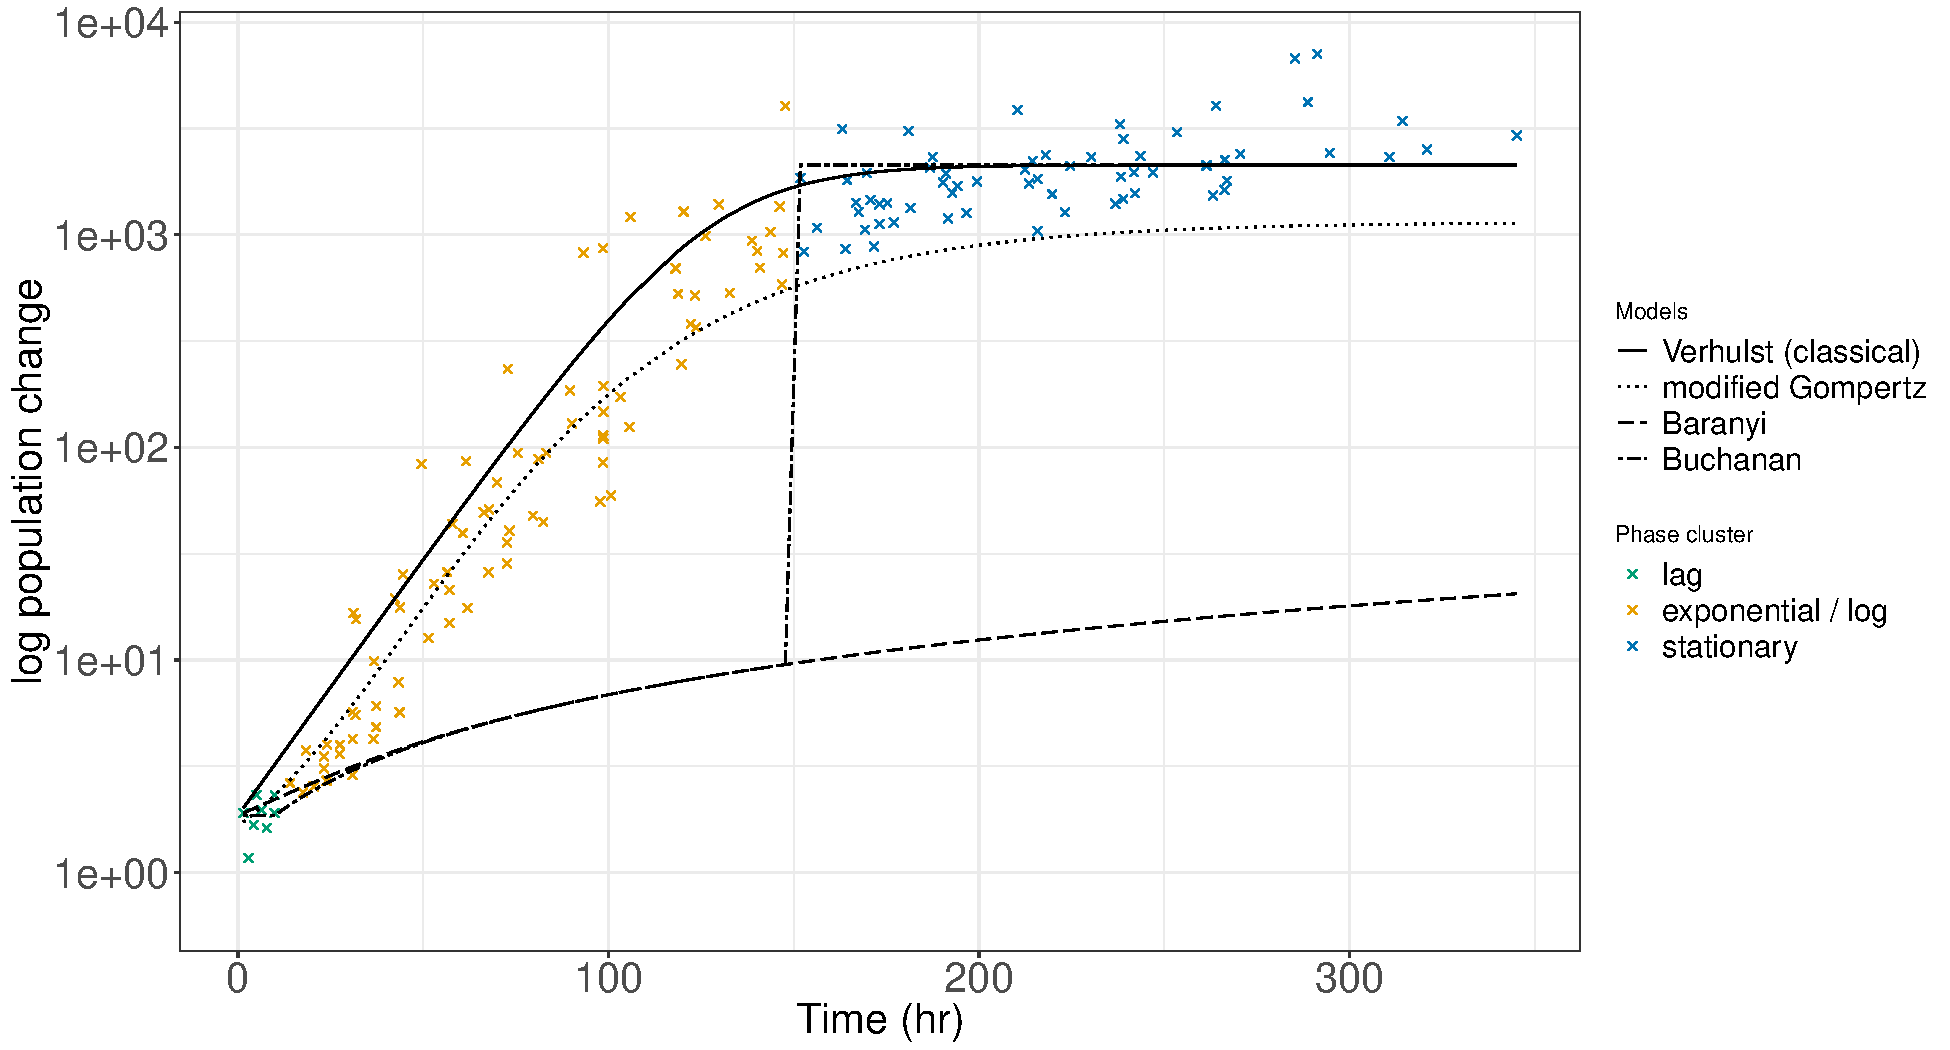
\includegraphics[width=\linewidth]{Log_data.pdf}\label{log-log}
		\caption{Log-Log graph showing four different models fitting on data of ``Population Change" against ``Experiment time" with points clustered into three main phases of sigmoid growth curve.}
	\end{figure}
	\section*{Discussion}
	\section*{Conclusion}
	\section*{Code and Data Availability}
	All \href{https://github.com/ph-u/CMEECourseWork_pmH/tree/master/MiniProject/code}{scripts} and \href{https://github.com/ph-u/CMEECourseWork_pmH/tree/master/MiniProject/data}{data} used for this report were publicity available at GitHub.
	\nocite{*}\printbibliography
\end{document}